\chapter{Uvod}


Ovaj završni rad dio je istraživanja koji se bavi analizom hrkanja. U okviru ovog rada, razvijen je sustav za prikupljanje zvučnih zapisa hrkanja, koji će se kasnije koristiti pri analizi. Budući da se istraživanje i snimanje provode u kliničkom okruženju, gdje postoje ograničenja nad uređajima koji nadziru i snimaju pacijente, potrebno je razviti neinvazivno softversko i hardversko rješenje koje će snimati i slati podatke na udaljenu lokaciju. Kao uređaj za snimanje zvuka odabran je mikrokontroler STM32WB5M koji će snimati zvučne zapise hrkanja i slati ih putem Bluetooth sučelja na računalo.  

U okviru ovog završnog rada razvijena je programska potpora za mikrokontroler STM32WB5M te je uspostavljeno BLE komunikacijsko sučelje između razvojnog sustava i osobnog računala s operacijskim sustavom Linux. Sučeljem se prenosi zvučni signal sniman MEMS mikrofonom s mikrokontrolera na računalo. Također je i razvijeno korisničko sučelje za pokretanje komunikacije, prijem i pohranu signala. Blok shema sustava prikazana je na Slici \ref{fig:shema}. 

\begin{figure}[ht]
	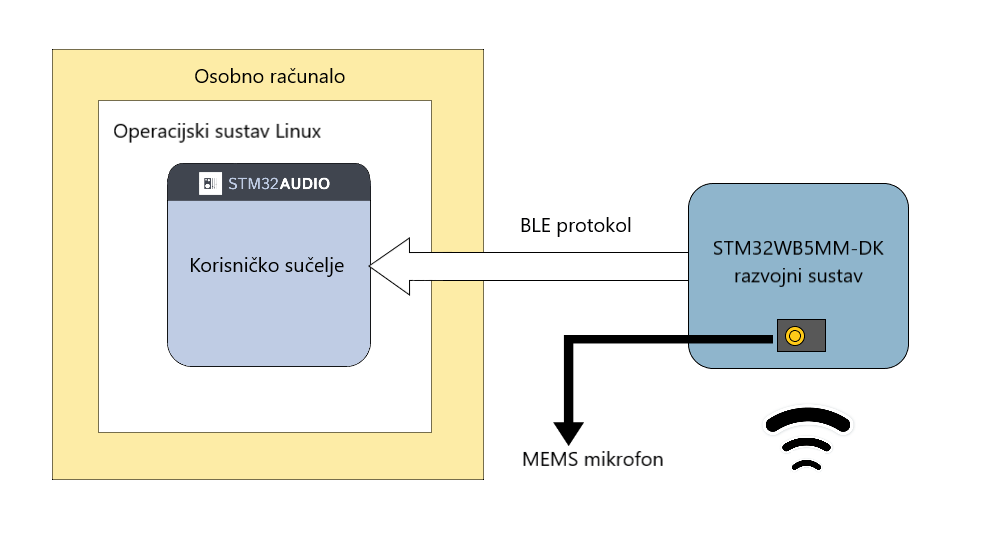
\includegraphics[width=\linewidth]{imgs/shema}
	\caption{Blok shema sustava}
	 \label{fig:shema}
\end{figure}

\eject